% Insufficient -> The extension is unrelated to the release engineering practices and focuses on an implementation aspect. The extension is trivial or irrelevant for the current project.
% Sufficient -> The report describes a meaningful extension to either the training pipeline, release pipeline, contribution process, or deployment. It does not have to cover more than one.
% Good -> The report contains a critical reflection on the existing design and provides a convincing argumentation of a current shortcoming and its negative effect.
% Very Good -> The presented solution is clearly addressing the described shortcoming. The report also includes a brief explanation of how the success could be measured objectively.
% Excellent -> The presented extension is general in nature. It is relevant and applicable beyond the context of the concrete project.

\section{Project State}
As is only natural, no project is only smooth sailing. Every design decision has its risks and pitfalls. In this section we therefore reflect on the current state of the project, discuss what went wrong and how to improve.
\subsection{Limitations}
% Critically reflect on the current state of your project and identify the point that you find the most critical/annoying/error prone. Equipped with the knowledge of the course.
% Describe the identified shortcoming and its effect. A convincing argumentation is crucial.
During development the biggest pitfall was definitely the Kubernetes provisioning. After many failed attempts trying minikube or k3d, finally k3s ended up working.

Furthermore, a limitation, which we have also previously mentioned is that fact that we have secrets in our docker images. We currently have this way of handling things to allow public access to the repository. In general, if we had restricted access to the application, we would probably have to instruct people how to change a configuration file with some credentials in order to get the system to work. Alternatively, we could maintain the current way of doing things, but add a step where we encrypt the secrets and decrypt them with a key we would provide to intended users.

This a development-related limitation, but right now, every time we update an image, the entire packages and libraries have to be downloaded. This is especially problematic for \texttt{model-service} as it's dependencies are around 1.5GB. We can instead cache the libraries and use docker to check whether there is a library cache on the machine and whether the versions of the dependencies match with the ones specified in the pipenv/poetry file. This would improve the download time of the image.

Another limitation however, is the way we store the machine learning model. Right now we use DVC Live to pull the model. This has the disadvantage of needing access to the DVC GitHub repository in order to get the model. It also requires having access to secrets in order to access the storage where DVC data is stored. This is a lot of unnecessary overhead, considering model-service only needs to download a copy of the model, which created a lot of problems during it's implementation.   

Focusing more on release engineering practices we notice the system's monitoring and experimentation capabilities are fairly limited. We do collect some useful metrics, such as the number of active requests, the total number of requests with corresponding histograms. However, in order to monitor the model itself more complex steps must be taken. \\
Regarding the experimentation, our pipeline does support multiple releases which we can use for A/B testing. However, this can be extended to support gradual rollouts. We have to provide additional configurations to Istio in order to support this.   

\subsection{Extension} % or refactoring
% • Describe and visualize a project refactoring/extension that improves the situation.
% • Link to information sources that provide useful information about the problem, inspiration for your solution, or concrete examples for its realization. We expect that you cite respectable sources (e.g., research papers; quality blogs like Medium; tool websites; or popular StackOverflow discussions).
% • Describe how you could test whether the changed design would solve the original shortcoming.
To mitigate the problem described in the previous section, we can migrate from using DVC live to and AWS s3 bucket. We can see the difference in the two approaches in Figure {\color{red}\ref{fig:fetch-model-workflows}}. The main advantage is that we no longer would need a secret to access the model, making the application more secure, since we wouldn't have to deal with the problem of secrets being stored in files as previously mentioned. The logic of uploading the model would be moved to the \texttt{model-training} component. We would know this would solve the initial problem, since no more secrets would be stored in images and also would create a more pronounced isolation layer between \texttt{model-service} and \texttt{model-training}. \\

Additionally, to improve ML monitoring, concept drift detection would be a great improvement. Currently, we can automatically train a model and deploy it. However, apart from the metrics we collect during training, we do not know how the model is performing over time, due to changes in data for example. A concept drift detector can solve this problem by monitoring the error rate of a model or the changes in the distribution of the data over time.  
. 

\begin{figure*}[h]
    \centering
    \begin{subfigure}[b]{0.45\linewidth}
        \centering
        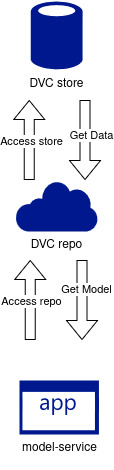
\includegraphics[width=0.35\linewidth]{images/original_fetch.jpg}
        \caption{Visualization of original workflows for fetching the model}
        \label{fig:libversion-workflow1}
    \end{subfigure}
    \hfill
    \begin{subfigure}[b]{0.45\linewidth}
        \centering
        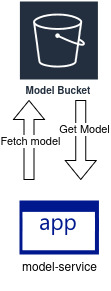
\includegraphics[width=0.35\linewidth]{images/improved_fetch.jpg}
        \caption{Visualization of improved workflow for fetching the model}
        \label{fig:libversion-workflow2}
    \end{subfigure}
    \caption{Side by side visualizations of \texttt{lib-version} workflows}
    \label{fig:fetch-model-workflows}
\end{figure*}
